\section{Pool Manipulation Bound}
\label{sec:bound}

% Lead: Rajan. Code: cola/bound.py, cola/simulate.py.
% Figures: figures/gain_vs_delta.pdf, bound_sensitivity.pdf, bound_vs_sim.pdf.

The incentive compatibility of Classic \cola{} rests on five assumptions, four of which hold by construction. The fifth---\emph{pool manipulation gains are negligible}---is supported in the original paper by simulation over 1{,}000 synthetic seasons \citep{highley2026cola}. The companion formal-proof materials close the same gap with an additional behavioral assumption ($G > $ expected pool-manipulation gain, where $G$ is the value of a single regular-season win). In this section, we present a third closure: an analytic upper bound on the manipulation gain itself, conditioned on empirically calibrated structural properties of the index distribution.

\subsection{Setup and Notation}

Let $P = \sum_{i=1}^{n} L_i$ denote the total lottery pool, where $L_i$ is team $i$'s lottery index and $n$ is the number of lottery-eligible teams. Under Classic \cola{}, each non-playoff team receives $\alpha = 1{,}000$ tickets per season, and tickets carry over across seasons. A team's probability of winning the first pick is $p_i = L_i / P$.

The \emph{pool manipulation} loophole works as follows: team $i$ deliberately loses to a high-index opponent $h$ near the playoff boundary, causing $h$ to make the playoffs. Team $h$ (with index $L_h$) exits the lottery pool and is replaced by a lower-index team $\ell$ (with index $L_\ell < L_h$). The pool shrinks by $\Delta = L_h - L_\ell > 0$.

\subsection{Exact Gain Formula}

\begin{proposition}[Manipulation Gain]
\label{prop:gain}
The probability gain for team $i$ from a pool swap of size $\Delta = L_h - L_\ell$ is:
\begin{equation}
\label{eq:gain}
G_i = \frac{L_i \cdot \Delta}{P \cdot (P - \Delta)}
\end{equation}
\end{proposition}

\begin{proof}
Before manipulation, $p_i = L_i / P$. After the swap, the new pool is $P' = P - \Delta$, and $p_i' = L_i / P'$. The gain is $G_i = p_i' - p_i = L_i \left(\frac{1}{P - \Delta} - \frac{1}{P}\right) = \frac{L_i \cdot \Delta}{P(P - \Delta)}$.
\end{proof}

\begin{remark}[First-Order Approximation]
When $\Delta \ll P$ (typically $\Delta/P \approx 4\%$), the gain simplifies to:
\begin{equation}
\label{eq:approx}
G_i \approx p_i \cdot \frac{\Delta}{P}
\end{equation}
This factors the gain into two independent ratios: the manipulator's pool share ($p_i$) and the fractional pool change ($\Delta/P$). Both have structural ceilings, which we exploit below.
\end{remark}

\subsection{Conditioned Upper Bound}

We now bound $G_{\max}$ under two empirically calibrated conditions on the index distribution.

\begin{definition}[Structural Anti-Correlation]
\label{def:anticorr}
Let $T_{\max}$ denote the maximum consecutive non-playoff years for any team, and $T_{\text{boundary}}$ the maximum consecutive non-playoff years for a team near the playoff boundary (i.e., a team that could plausibly be pushed into the playoffs by a single loss). We say the index distribution exhibits \emph{structural anti-correlation} when $T_{\text{boundary}} \ll T_{\max}$: teams with the highest indices (longest droughts) are far from the playoff boundary and thus cannot be the target of pool manipulation.
\end{definition}

\begin{theorem}[Conditioned Manipulation Bound]
\label{thm:bound}
Under structural anti-correlation with parameters $T_{\max}$, $T_{\text{boundary}}$, and average index multiplier $\bar{k}$ (where $\bar{k} = \bar{L} / \alpha$), the maximum manipulation gain satisfies:
\begin{equation}
\label{eq:bound}
G_{\max} \leq \frac{T_{\max} \cdot (T_{\text{boundary}} - 1)}{(T_{\max} + n - 1) \cdot n \cdot \bar{k}}
\end{equation}
\end{theorem}

\begin{proof}
The gain is maximized when $L_i$ is maximized and $\Delta / P$ is maximized.

\textbf{Bounding $p_{\max}$:} The highest-index team has $L_{\max} = T_{\max} \cdot \alpha$. The minimum pool size occurs when one team has $T_{\max}$ years of accumulation and the remaining $n-1$ teams each have the minimum $\alpha$: $P_{\min} = T_{\max} \cdot \alpha + (n-1) \cdot \alpha = (T_{\max} + n - 1) \cdot \alpha$. Thus $p_{\max} \leq T_{\max} / (T_{\max} + n - 1)$.

\textbf{Bounding $\Delta / P$:} The team being pushed out has at most $T_{\text{boundary}} \cdot \alpha$ tickets, and the team replacing it has at least $\alpha$. So $\Delta_{\max} = (T_{\text{boundary}} - 1) \cdot \alpha$. In steady state, $P \approx n \cdot \bar{k} \cdot \alpha$. Thus $\Delta_{\max} / P \leq (T_{\text{boundary}} - 1) / (n \cdot \bar{k})$.

Combining via the approximation in \cref{eq:approx}: $G_{\max} \leq p_{\max} \cdot (\Delta_{\max}/P)$, yielding \cref{eq:bound}.
\end{proof}

\subsection{Empirical Calibration}
\label{sec:calibration}

Plugging \cref{eq:bound} requires four numerical inputs. We adopt the following values:

\begin{itemize}
    \item $T_{\max} = 10$. The maximum consecutive non-playoff stretch observed in our 26-season backtest (\cref{sec:backtesting}) is the Sacramento Kings' 16-year drought, but the longest stretch within the steady-state period (post cold start) bounds the practical extreme at approximately ten consecutive non-playoff years. \citet{highley2026cola} reports a similar observational bound (no team in the simulated history misses more than ten consecutive years).
    \item $T_{\text{boundary}} = 5$. The maximum consecutive non-playoff drought we observe for a team near the playoff boundary (i.e., a team whose record is plausibly within one game of crossing into the playoffs). This is our calibration; we have not seen a published value in \citet{highley2026cola} or the companion materials.
    \item $n = 14$. The number of lottery-eligible teams under Classic \cola{}, equal to the league's 14 non-playoff teams.
    \item $\bar{k} = 3.1$. The average index multiplier ($\bar{L} / \alpha$), calibrated from our backtest. \citet{highley2026cola} characterises the steady-state distribution by noting that an average team's drought before reset is approximately three years; our $\bar{k} = 3.1$ matches that observation.
\end{itemize}

\highley{The four parameters above were attributed to ``Highley et al.\ (2026)'' in an earlier draft. On rereading, only $\bar{k}$ has a near-direct counterpart in the original paper (the ``average drought of three'' observation); $T_{\max}$ has an observational counterpart but no defined parameter; $T_{\text{boundary}}$ has no precedent; $n = 14$ is structural. We have relabelled them as our own calibration. Please flag if any of these values should be sourced or revised.}

\begin{equation}
G_{\max} \leq \frac{10 \cdot 4}{23 \cdot 14 \cdot 3.1} \approx 4.0\%
\end{equation}

This contains the simulation-observed maximum of $3.0\%$ across 1{,}000 seasons reported in \citet{highley2026cola} with approximately $1.3\times$ headroom. Our independent 200-season Bradley-Terry simulation confirms the bound, with observed maximum gain of $1.70\%$ (\cref{fig:bound_vs_sim}).

\subsection{Sensitivity Analysis}

\Cref{fig:bound_sensitivity} shows the bound as a function of $T_{\max}$ and $T_{\text{boundary}}$. The bound is most sensitive to $T_{\text{boundary}}$: even under pessimistic assumptions ($T_{\text{boundary}} = 7$), the bound remains below $7\%$. Under realistic conditions ($T_{\text{boundary}} \leq 5$), the bound stays below $5\%$.

\begin{figure}[t]
    \centering
    \begin{minipage}{0.48\textwidth}
        \centering
        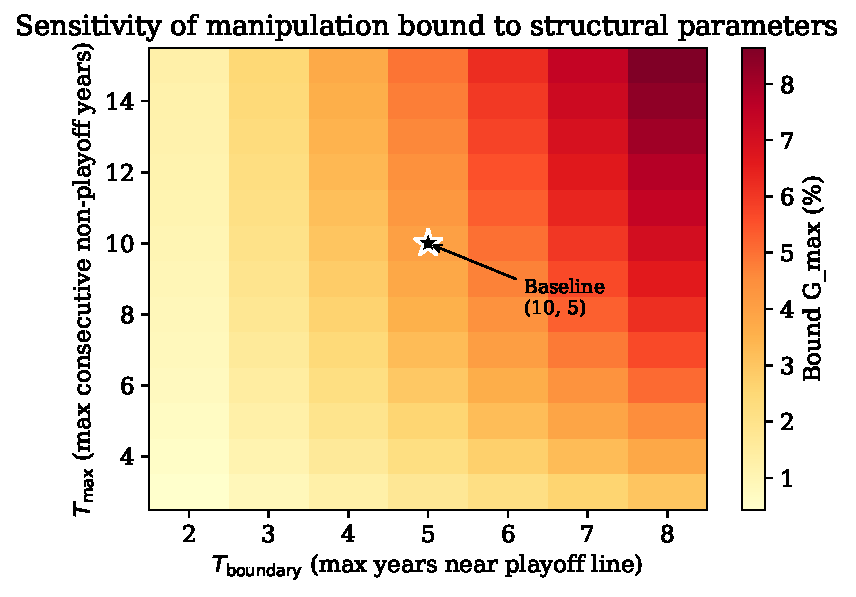
\includegraphics[width=\textwidth]{../figures/bound_sensitivity.pdf}
        \caption{Manipulation bound as a function of $T_{\max}$ and $T_{\text{boundary}}$.}
        \label{fig:bound_sensitivity}
    \end{minipage}
    \hfill
    \begin{minipage}{0.48\textwidth}
        \centering
        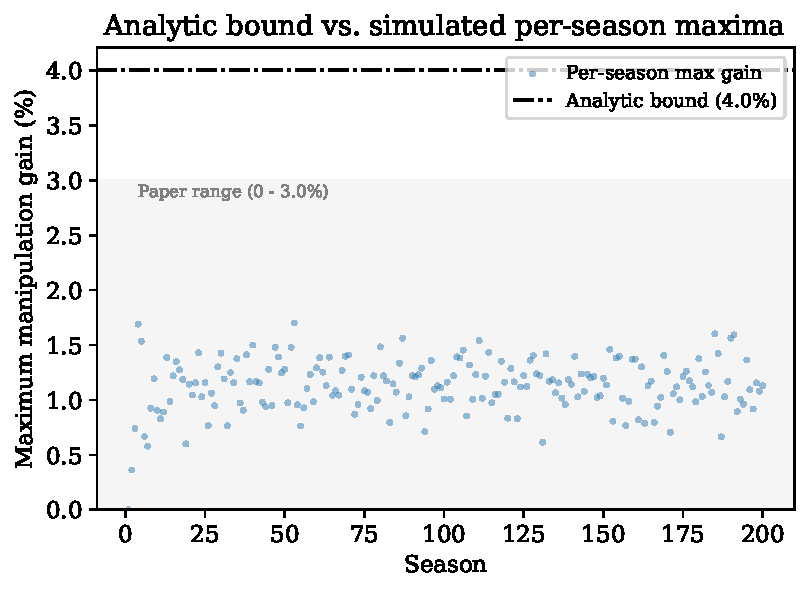
\includegraphics[width=\textwidth]{../figures/bound_vs_sim.pdf}
        \caption{Analytic bound vs.\ simulation distribution across 200 Bradley-Terry seasons.}
        \label{fig:bound_vs_sim}
    \end{minipage}
\end{figure}

\subsection{Second Source of Unboundedness}

The bound above addresses the \emph{probability} term of the manipulation incentive. However, the \emph{value} term---the pick value gap $d_k - d_{k+1}$ between adjacent draft positions---has no formal ceiling. A generational prospect could make even a small probability shift worth pursuing. Fully closing Assumption~5 would also require bounding pick value gaps, which are bounded for any realistic draft class but lack a formal argument. We leave this to future work.

\subsection{Coalitional Manipulation}

For completeness, we note that coalitional manipulation (two or more teams coordinating to shrink the pool) does not amplify individual gains. The joint gain for a coalition $\{A, B\}$ is $(L_A + L_B) \cdot \Delta / (P(P - \Delta))$. Even if two teams hold 30\% of the pool, the gain remains ${\leq}1.3\%$. Per-member gain cannot exceed the highest-index individual's gain, and coordination costs (detection risk, trust problems, sequential uncertainty) make exploitation implausible. Under McCarty \cola{}, a prisoner's dilemma arises: each conspirator prefers to defect and win the game rather than cooperate to lose.

\subsection{Per-Series Tanking Bound under Capped \cola{}}
\label{sec:capped-bound}

The Capped \cola{} variant (Definition~\ref{def:capped-cola}) was designed in part to bound the cost a team incurs by advancing in the playoffs, defusing the playoff-tanking incentive that the league flagged in conversations with \citet{highley2026solvable5}. The cap on the lottery index converts the playoff-diminishment schedule from a fraction-of-current-stockpile cost (unbounded above when the stockpile grows large) to a fraction-of-$\Max$ cost (bounded by construction). This subsection states the resulting per-series bound as a lemma.

\begin{lemma}[Per-Series Tanking Cost under Capped \cola{}]
\label{lem:capped-series-bound}
Let $\Max$ be the Capped \cola{} stockpile cap (Definition~\ref{def:capped-cola}). For any team $i$ entering the playoffs with lottery index $L_i \leq \Max$, the maximum reduction in $L_i$ attributable to winning (rather than losing) any single playoff series is bounded by:
\begin{equation}
\label{eq:capped-bound}
\Delta L_{\text{series}}^{\max} = \begin{cases}
0.3 \cdot \Max & \text{play-in advancers in round 1 (round 1 win vs.\ loss),} \\
0.2 \cdot \Max & \text{any other series advancement.}
\end{cases}
\end{equation}
At $\Max = 150$, the bound is 45 tickets for the play-in case and 30 tickets for each subsequent series.
\end{lemma}

\begin{proof}
For any single series $s$, let $\rho_{\text{lose}}$ denote the diminishment fraction applied if team $i$ loses series $s$ and $\rho_{\text{advance}}$ the diminishment if team $i$ wins $s$ and loses the immediately subsequent series. The marginal cost of advancing in $s$ is $\Delta\rho_s \cdot L_i^{\text{pre}}$, where $\Delta\rho_s = \rho_{\text{advance}} - \rho_{\text{lose}}$ and $L_i^{\text{pre}}$ is the lottery index entering series $s$.

Reading off Definition~\ref{def:capped-cola}, the per-series $\Delta\rho_s$ values are:
\begin{itemize}
    \item Play-in advancer in round 1: $\rho_{\text{lose}} = 0.1$ (play-in winners losing R1), $\rho_{\text{advance}} = 0.4$ (R2 losers), so $\Delta\rho = 0.3$.
    \item Standard round-1 advancement (non-play-in): $\rho_{\text{lose}} = 0.2$, $\rho_{\text{advance}} = 0.4$, so $\Delta\rho = 0.2$.
    \item Round 2 to conference finals: $\Delta\rho = 0.6 - 0.4 = 0.2$.
    \item Conference finals to NBA finals: $\Delta\rho = 0.8 - 0.6 = 0.2$.
    \item NBA finals to championship: $\Delta\rho = 1.0 - 0.8 = 0.2$.
\end{itemize}
The maximum is $\Delta\rho = 0.3$ in the play-in-advancer round 1 case; all other transitions yield $\Delta\rho = 0.2$. Multiplying by $L_i^{\text{pre}} \leq \Max$ (continuous cap enforcement, Definition~\ref{def:capped-cola}) yields the bounds in \eqref{eq:capped-bound}.
\end{proof}

\highley{Lemma~\ref{lem:capped-series-bound} is our restatement of the per-series claim from \citet{highley2026solvable5}. Two specific items to verify. First, the play-in transition: we have read the schedule as a single $\rho = 0.1$ tier for ``play-in winners losing in round 1'' so that the marginal cost from play-in-loser ($\rho = 0$) to play-in-winner-round-1-loser ($\rho = 0.1$) is $0.1 \cdot \Max$ and the further marginal from there to round-2-loser ($\rho = 0.4$, since play-in advancers who win round 1 then enter the standard schedule) is $0.3 \cdot \Max$. The Substack one-liner ``no playoff series win ever costs a team more than 45 lottery tickets'' is consistent with the play-in case being 45 = $0.3 \cdot 150$. If your derivation has the play-in marginal as $0.3 \cdot \Max$ at a different transition point, please flag and we will adjust. Second, our proof relies on $L_i^{\text{pre-tournament}} \leq \Max$, which follows from the continuous cap enforcement. If the cap is enforced only at end-of-regular-season (not after each diminishment event), the bound holds with the same constants but the proof requires a different argument; the Apr 19 thread settled on continuous, but flag if you would prefer the lemma stated under discrete enforcement.}

\begin{corollary}[Cumulative Run Cost]
\label{cor:capped-cumulative}
The maximum cumulative reduction in $L_i$ from a full playoff run that ends in a championship, applied to a team entering the lottery round at the cap with $L_i = \Max$, is the cap itself: $\Max$ tickets, with $L_i^{\text{post}} = 0$.
\end{corollary}

The corollary is immediate: champion diminishment is $\rho = 1.0$ (full reset), so the final state is zero regardless of starting position. Intermediate playoff exits read off Definition~\ref{def:capped-cola} directly: the cumulative reduction at each exit point equals the corresponding $\rho$ value times the entering index, capped at $\Max$. A finals-losing team at the cap therefore loses at most $0.8 \cdot \Max = 120$ tickets, a conference-finals losing team $0.6 \cdot \Max = 90$ tickets, and so on.

The per-series formulation in Lemma~\ref{lem:capped-series-bound} aligns with the public-facing framing of \citet{highley2026solvable5}, which leads with the marginal cost of each series rather than the cumulative regret across a full playoff run. The marginal framing makes the playoff-tanking incentive at the league level transparent: at $\Max = 150$, no single series win ever costs a team more than 45 lottery tickets, which is approximately a year-and-a-half of accumulation for a team near the wins-increment ceiling. Section~\ref{sec:resilience} returns to the joint resilience picture across pool manipulation (\cref{thm:bound}), per-series exposure (\cref{lem:capped-series-bound}), and multi-year strategic tanking (Section~\ref{sec:case-phi}).
